\chapter{Etablierung Agiler Praktiken}
\label{agilepractices}

% - erkenntnisreichster Teil der Arbeit!
% - Erarbeitung von verwendeten agilen Praktiken
% - Evaluation hinsichtlich ihrer Anwendbarkeit bei den vorher erarbeiteten Problemfeldern

Im nachfolgenden Kapitel soll der zweite wesentliche Schwerpunkt der erarbeitet werden. Nachdem in \ref{problemfields} grundsätzliche Problemfelder innerhalb der Digitalen Transformation von Großunternehmen untersucht wurden, sollen nun anhand eines zweiten SLR agile Methoden gefunden werden, die diesen Problemfeldern begegnen können. Als erster Schritt soll wiederum das methodische Vorgehen erläutert werden, wonach eine Reihe von Literatur für das zweite SLR zusammengestellt wurde. Anhand dieser werden agile Methoden extrahiert, die vermehrt innerhalb des Transformationsprozesses eingesetzt wurden. Diese sollen anschließend kurz dargestellt und hinsichtlich ihrer Anwendbarkeit bei bestimmten Problemfeldern evaluiert werden. Als Ergebnis dessen sollen als generelles Resultat der vorliegenden Arbeit Best Practices für den Einsatz agiler Methoden in der Digitalen Transformation ausgearbeitet werden. Das nachfolgende Literaturreview wird durch das Akronym \textit{SLR 2} abgekürzt.

\section{Methodisches Vorgehen}
\label{agilepractices:methods}

% - genaue Darstellung über Vorgehen in der SLR + Metastudie: 
% - Suchmethodik, Keywords, Kriterien, Auswahlprozes ...
% + Schema der Evaluation (Problemfelder)
% https://docs.google.com/document/d/1j8hegu3FgQk2fPMVjo8IUPWIXwNjlZjT42rHxg7KZ1I/edit

Das Vorgehen in den folgenden Ausführungen teilt sich in zwei wesentlichen Unterpunkten. Zunächst soll, ähnlich dem SLR 1 in \ref{problemfields}, ein systematisches Literaturreview mit Metastudiencharakter vorgenommen werden. Die Vorgehensweise ähnelt der des ersten SLR, etwaige Besonderheiten werden nachfolgend aufgeführt. Der zweite  methodische Teil beinhaltet die Evaluation der erarbeiteten agilen Methoden. Dafür soll ebenfalls nachfolgend ein Evaluationsschema skizziert werden.

\subsection{Systematisches Literaturreview}

Im Vorfeld der Literatursuche wurde zunächst eine Suchstrategie erstellt. Diese ähnelt der im \ref{problemfields:methods} dargestellten, \ref{fig:suchstrategie} illustriert somit ebenfalls die Strategie zur Suche relevanter Literatur für SLR 2. Für die zweite Literatursuche wurden die verwendeten Keywords verändert. Wiederrum wurden diese in Suchketten zusammengefasst, welche sich jeweils für englische und deutsche Literaturdatenbanken unterscheiden. Die genutzten Suchketten werden in \ref{tab:keywordsslr2} aufgeführt. An dieser Stelle sei wieder zu erwähnen, dass die Syntax zwischen verschiedenen Suchmaschinen unterscheiden kann. Die Übersicht dient der Allgemeinheit.

\begin{table}[ht]
	\centering
	\caption{Übersicht Keyword-Suchketten SLR 2}
	\begin{tabular}{|p{7cm}|p{7cm}|}
		\hline
		\textbf{Deutsche Keywords}& \textbf{Englische Keywords} \\
		\hline
		agile+transformation+fallstudie OR digitale+transformation+agil OR agile+organisation+fallstudie   & agile+transformation+case OR digital+transformation+agile OR agile+organization+case \\
		\hline
	\end{tabular}
	\label{tab:keywordsslr2}
\end{table}

Auch die verwendeten Literaturdatenbanken bzw. Suchmaschinen ähneln denen des ersten SLR. Wiederrum wurde eine Übersicht für die Anzahl an Treffern der Keywords in den jeweiligen Suchmaschinen aufgestellt. Diese findet sich in \ref{tab:suchmaschinenslr2}. Für die Suchmaschine \textit{ResearchGate} konnte auch für die zweite Literatursuche keine Angabe zu Keyword-Treffern gemacht werden. Eine kurze Erklärung findet sich in \ref{problemfields:methods}.

\begin{table}[ht]
	\centering
	\caption{Übersicht Literatursuchmaschinen SLR 2}
	\begin{tabular}{|p{5cm}|p{7cm}||p{3cm}|}
		\hline
		\textbf{Datenbank/Bibliothek}& \textbf{URL} &  \textbf{Treffer Keywords  (summiert)} \\
		\hline
		IEEE Xplore & \url{https://ieeexplore.ieee.org} & 316 \\
		(Online) - Bibliothek Hochschule Harz & \url{https://opac.lbs-magdeburg.gbv.de/DB=4/LNG=DU} & 4 \\
		(Online) - Bibliothek Technische Universität Berlin  & \url{https://www.ub.tu-berlin.de/literatur-suchen}& 5 \\
		Google Scholar &  \url{https://scholar.google.de}  & 23.500 \\
		Scopus & \url{https://www.scopus.com} & 1.491 \\
		ResearchGate & \url{https://www.researchgate.net} &Keine Angabe vorhanden \footnotemark \\ 
		ACM Digital Library & \url{https://dl.acm.org} & 251.254 \\
		\hline
	\end{tabular}
	\label{tab:suchmaschinenslr2}
\end{table}

Die andauernde Literatursuche wurde wieder mithilfe einer Forwards-Backwards-Suche unterstützt. Die angestrengte Suche erzielte somit wieder eine große Menge an potenzieller Literatur zur Thematik. Somit war auch hier eine Filterung der Ergebnisse mithilfe eines Auswahlprozesses notwendig. Dieser gleicht ebenfalls der im ersten SLR. Somit zeigt \ref{fig:auswahlprozess} in \ref{problemfields:methods} eben diesen. 

Auch für dieses Auswahlprozedere wurden eine Reihe von Ein - und Ausschlusskriterien definiert. Diese werden nachfolgend in \ref{tab:criteriaslr2}. Auch hier zeigen sich verständlicherweise Parallelen zum ersten SLR. Wichtig hier zu erwähnen sei, dass innerhalb der Publikationen ein klarer Bezug zu agilen Methoden im Transformationsprozess erkennbar sein muss. Hierbei reicht nicht nur die Nennung einzelner Methoden, es muss klar ersichtlich sein, welchen Beitrag diese zum Veränderungsprozess beigetragen werden. Dies ist gerade wichtig im Hinblick auf die nachfolgende Evaluation. Im Bezug auf Internationalität und Branchenzugehörigkeit wurden keine Einschränkungen getroffen.

\begin{table}[ht]
	\centering
	\caption{Ein - und Ausschlusskriterien SLR 2}
	\begin{tabular}{|p{4cm}|p{8cm}|}
		\hline
		\textbf{Kriterium}& \textbf{Erklärung}  \\
		\hline
		Empirik & Literatur muss eine Fallstudie oder Studie sein. Fachliteratur auch dann möglich, wenn klarer Bezug auf Agile Organisationsentwicklung in Großunternehmen \\
		Wissenschaftlichkeit & Methodik der  Fallstudie oder Studie muss klar erkennbar sein \\
		Kontext 1 & inhaltlich Digitale Transformation in Großunternehmen; Mittelständische nur dann, wenn relevant für größeren Kontext \\
		Kontext 2 & Nutzung klarer, spezifischer agiler Methoden im Transformationsprozess \\
		Sprache & deutsch oder englisch \\
		Aktualität & ab 2014 - heute  \\
		\hline
	\end{tabular}
	\label{tab:criteriaslr2}
\end{table}

Durch eine zweite Literatursuche konnte wieder eine große Menge relevanter Literatur, in diesem Falle nicht vollumfänglich Fallstudien, für die nachfolgenden Untersuchungen erschlossen werden. Zwischen beiden Untersuchungen gab es in der Ergebnismenge Überschneidungen, da manche Fallstudien ebenfalls die Nutzung agiler Methoden einschlossen. Dies ist deshalb sehr interessant, weil dadurch direkt Handlungsfelder agiler Methoden hinsichtlich der geschilderten Problemfelder erkennbar wurden. Insgesamt konnten nach dem Auswahlprozess \textit{32} Publikationen für die weitere Verwendung gefunden werden. Darunter beinhalten 29 davon Fallstudien, 3 sind Fachliteratur. Die Anzahl der Fallstudien konnte diesmal auf über \textit{180} aus verschiedenen Branchen gezählt werden. An den eingeschlossenen Studien nahmen insgesamt über 1500 Offizielle aus Großunternehmen teil. 

\subsection{Evaluation}

Als zweiter methodischer Teil wurde eine Evaluation der zuvor erarbeiteten agilen Methoden vorgesehen. Diese soll nach einem klaren Schema erfolgen, welches nachfolgend erläutert werden soll. 

Die vorgenommene Evaluation wurde nach Vorbild eines Leitfadens des Bundesministerium für Ernährung und Landwirtschaft erstellt \footnote{Leitfaden Evaluation, \newline online: \url{https://www.in-form.de/fileadmin/Dokumente/Materialien/IN_FORM_Leitfaden_Evaluation.pdf}}. Dieser beinhaltet insgesamt 6 Phasen, welche in \ref{fig:evaluation} dargestellt werden. Zu jeder Phase zeigt die Abbildung ebenfalls das Resultat im Bezug auf die  vollzogene Evaluation. 

Zunächst sollte das Ziel der Evaluation dekliniert werden. Im Vordergrund stand hierbei ganz klar die Lösung der in \ref{problemfields} erarbeiteten Problemfelder. Anschließend wurde der  Evaluationsgegenstand bestimmt. Dieses findet sich in der mithilfe des SLR 2 gefundenen agilen Praktiken bzw. Methoden. Somit setzt sich das zu betrachtende Untersuchungsfeld der Evaluation aus einer Beziehung zwischen Problemfelder der Digitalen Transformation und agilen Methoden zusammen.

\begin{figure}[H]
	\centering
	\fbox{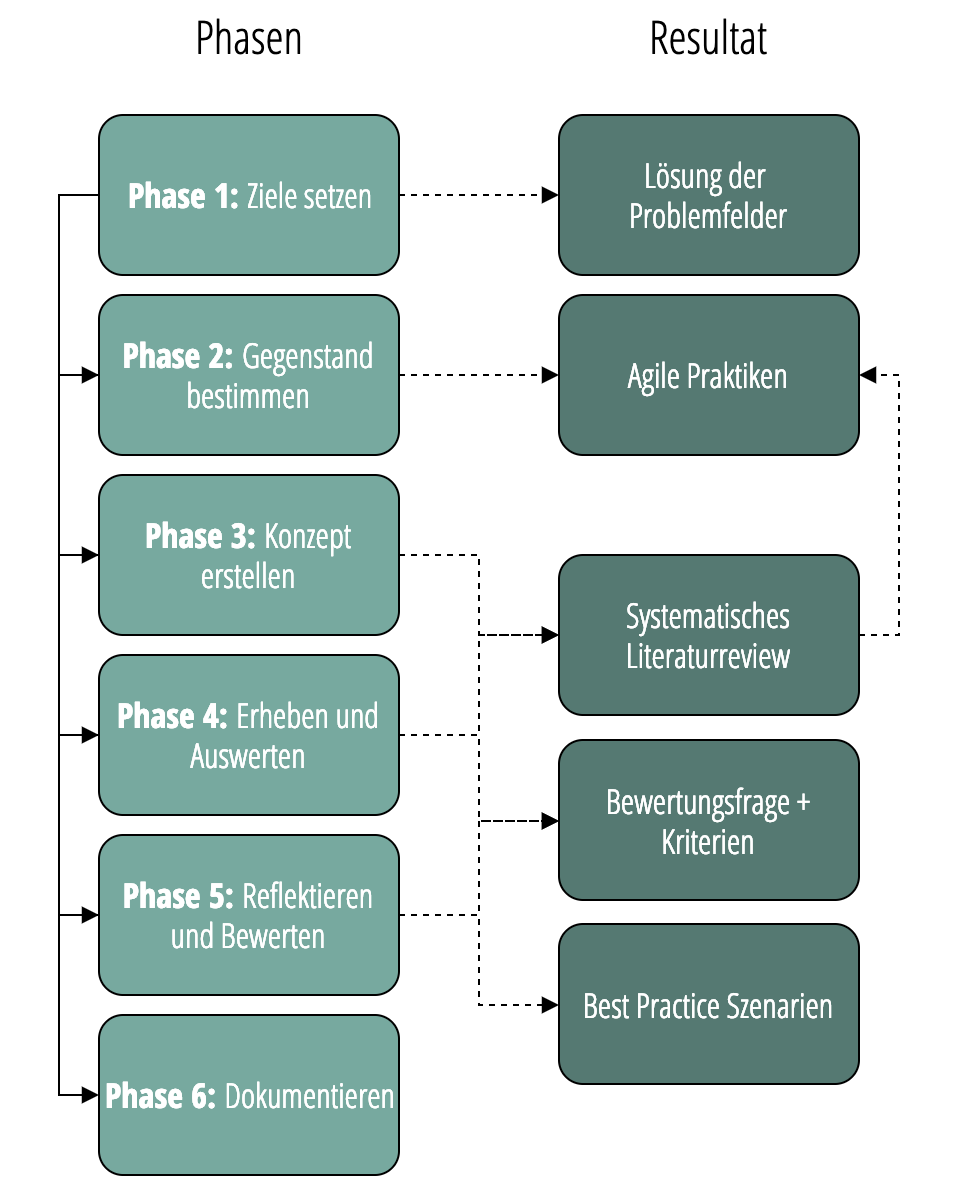
\includegraphics[width=0.6\linewidth]{pics/evaluation}}
	\caption[Darstellung Evaluationsprozess]{Darstellung Evaluationsprozess (eigene Darstellung)}
	\label{fig:evaluation}
\end{figure}

Phase 3 beinhaltet den wichtigsten Punkt der Evaluation. Hierbei wurde eine genaue \textit{Evaluationsfrage} erstellt: \textit{Welche vorher definierten Problemfelder können mithilfe welcher agilen Methode angegangen werden?}. Zum Evaluationskonzept wurden zudem Kriterien zur Beantwortung der Frage bezüglich einer jeden agilen Methode gestellt. Wichtig ist hierbei, dass die Bewertung immer auf Grundlage \textit{klarer, qualitativer Aussagen} aus der in SLR 2 gefundenen Literatur beziehen muss. Eine agile Methode gilt also genau dann als anwendbar auf ein bestimmtes Problemfeld, wenn sich dies durch eine Aussage innerhalb einer Publikation belegen lässt. Somit wurden die Suchobjekte aus SLR 2 als Bewertungsgrundlage für die dargestellte Evaluation gewählt.  Es lässt sich erkennen, dass die Bewertung auf Grundlage rein qualitativer Daten beruht.

Phase 5 und 6 finden sich im vorliegenden Kapitel wieder. Systematisch soll für jede aufgeführte agile Methode eine kurze Darstellung platziert werden und jeweils anschließend die Bewertung auf Grundlage der Aussagen vorgenommen werden. Als Ergebnis dessen werden Best Practice Szenarien für den Einsatz der einzelnen agilen Methoden erstellt, um zusammenfassend darzustellen, in welchem Rahmen sich die Methoden einsetzen lassen.


\section{Literaturübersicht}

% - tabellarische Übersicht, Fallstudien + allgemeine Sekundäre Literatur
% - Inhaltsangabe jeder Arbeit (Zusammenfassung)

\todo{siehe Tabelle 5-7 im Anhang}

\todots

\section{Einsatz agiler Praktiken im Unternehmen}

% - Ergebnisse der SLR - Auflistung der genutzten Methoden

\todo{siehe Tabelle 8  und 9 im Anhang}

\begin{table}[ht]
	\centering
	\caption{Auswertung Nutzung agiler Methoden (kurz)}
	\begin{tabular}{|c|c|}
		\hline
		\textbf{Agile Methode}& \textbf{Anzahl Nennungen} \\
		\hline
		Scrum                          & 17               \\
		Design Thinking                & 10               \\
		DevOps                         & 8                \\
		Kanban                         & 6                \\
		XP                             & 5                \\
		SAFe                           & 4                \\
		Digital Innovation Lab         & 4                \\
		Minimum Valuable Product (MVP) & 2                \\
		Squads and Tribes              & 2                \\
		LeSS                           & 1                \\
		Unified Process                & 1                \\
		Communities of Practice        & 1                \\
		Holacracy                      & 1                \\
		Culture Book                   & 1                \\
		Corporate Startups             & 1                \\
		Agile Modelling                & 1                \\
		Usability Driven Development   & 1                \\
		Lean Startup                   & 1               \\
		\hline
	\end{tabular}
	\label{tab:clusteringagileshort}
\end{table}

\todots

\section{Darstellung und Evaluation verschiedener agiler Methoden}

% - systematisch: erst Definition der Methode, dann Evaluation im Bezug auf die Problemfelder
% - siehe Key findings: https://docs.google.com/document/d/1QayCknP1SgspsPvXlU_FR5u0h2fNzhfQshNOrAuTiB8/edit

\todots

\subsection{Scrum}

\todots

\subsection{Design Thinking}

\todots

\subsection{DevOps}

\todots

\subsection{Kanban}

\todots

\subsection{XP}

\todots

\subsection{SAFe}

\todots

\subsection{Digital Innovation Lab}

\todots

\subsection{Minimum Valuable Product}

\todots

\subsection{Squads and Tribes}

\todots


\section{Formulierung agiler Best Practice Szenarien}

% - Erstellung von Thesen für Best-Practice Szenarien (im Bezug auf allen Ergebnissen von vorher, vor allen auch 4.3)

\todots


